\documentclass[12pt]{article}
\usepackage[top=1in,bottom=1in,left=1in,right=1in]{geometry}
\usepackage{alltt}
\usepackage{array}	
\usepackage{graphicx}
\usepackage{tabularx}
\usepackage{verbatim}
\usepackage{setspace}
\usepackage{listings}
\usepackage{amssymb,amsmath, amsthm}

\title{SOEN331: Introduction to Formal Methods\\for Software Engineering\\
Assignment 2 on Extended Finite State Machines}
\author{Martin Marcos 40041398,\\ Samantha Guillemette 26609198,\\ Deepkumar Patel 40096716  }

\date{\today}

\begin{document}
\begin{spacing}{1.5}

\maketitle

\section{Driver-less car system formal specification}

\noindent The EFSM of the driver-less car system is the tuple $S = (Q, \Sigma_1, \Sigma_2, q_0, V, \Lambda)$, where\\

\noindent $Q = \{idle, parked~mode, manual~mode, cruise~mode, marked~mode, panic~mode\}$\\
\noindent $\Sigma_1 = \{start, cruise~signal, switch, arrived, unforseen,panic~off, off\}$\\
\noindent $\Sigma_2 = \{lock, unlock, beep\}$\\
\noindent $q_0: idle$\\
\noindent $V: destination = \{set, no\}$\\
\noindent $\Lambda$: Transition specifications\\
\indent 1. $\rightarrow idle$\\
\indent 2. $idle \xrightarrow {\text { start }} parked mode$\\
\indent 3. $parked~mode  \xrightarrow {\text { off }} off?$\\
\indent 4. $parked~mode  \xrightarrow {\text { cruise signal [no dest] }} manual~mode$\\
\indent 5. $parked~mode  \xrightarrow {\text { cruise signal [set dest] / beep }} cruise~mode$\\
\indent 6. $manual~mode  \xrightarrow {\text { cruise signal [set dest] }} cruise~mode$\\
\indent 7. $cruise~mode  \xrightarrow {\text { switch }} manual~mode$\\
\indent 8. $cruise~mode  \xrightarrow {\text { arrived }} parked~mode$\\
\indent 9. $cruise~mode  \xrightarrow {\text { unforseen }} panic~mode$\\
\indent 10. $manual~mode  \xrightarrow {\text { stop }} marked~mode$\\
\indent 11. $panic~mode  \xrightarrow {\text { panic off / hazard off}} manual~mode$\\


\noindent The UML state diagram is shown in Figure~\ref{fig:main-system-fig}.

\newpage

\section{UML state diagrams}

\begin{figure}[h!]
	\centering
		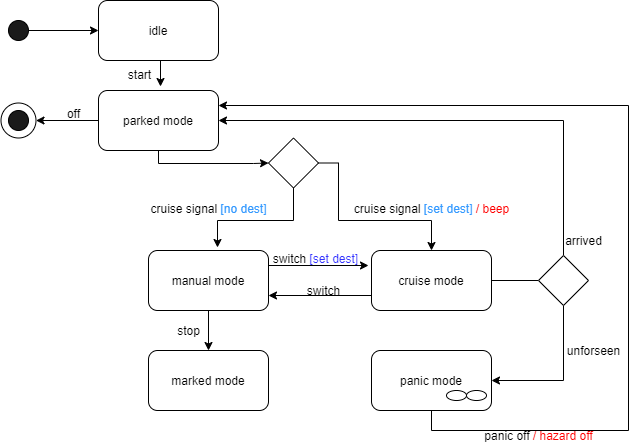
\includegraphics[width=0.8\textwidth]{./A2_Figures/4.1-Main-System.png}
		  \caption{Main System.}
  \label{fig:main-system-fig}
\end{figure}

\end{spacing}


\end{document}
